\chapter{初等関数と暗記すべき公式}
\label{ch:tb-functions}

この章は暗記が中心である。
公式そのものが問われることは少ないが、公式を思い出せないと
微分・積分の問題は最初の一行で止まる。

\section{指数関数と対数関数}

\begin{definition}{指数関数と対数関数}{tb-exp-log}
$a>0$, $a\ne1$ に対し $a^x$ を指数関数、その逆関数を $\log_a x$ と書く。
底が $e=2.718\ldots$ のときを\textbf{自然対数}といい、本書では単に $\log x$ と書く。
定義域は $x>0$ である。
\end{definition}

\begin{proposition}{指数法則と対数法則}{tb-exp-log-laws}
\[
a^{x+y}=a^xa^y,\qquad
(a^x)^y=a^{xy},\qquad
a^{-x}=\frac1{a^x},
\]
\[
\log(xy)=\log x+\log y,\qquad
\log\frac xy=\log x-\log y,\qquad
\log x^r=r\log x.
\]
また底の変換は $\log_a x=\dfrac{\log x}{\log a}$ である。
\end{proposition}

\begin{definition}{一般の冪 $x^{f(x)}$}{tb-general-power}
$x>0$ のとき、指数が変数であっても
\[
x^{f(x)}=\exp\bigl(f(x)\log x\bigr)
\]
と定める。$x^{\sin x}$ のような関数は、この形へ直してから微分する。
\end{definition}

\section{三角関数}

\begin{definition}{三角関数と、その逆数の三つ}{tb-trig-definition}
単位円上の角 $\theta$ に対する $\sin\theta$, $\cos\theta$ から
\[
\tan\theta=\frac{\sin\theta}{\cos\theta},\qquad
\sec\theta=\frac1{\cos\theta},\qquad
\csc\theta=\frac1{\sin\theta},\qquad
\cot\theta=\frac{\cos\theta}{\sin\theta}=\frac1{\tan\theta}
\]
と定める。それぞれ\textbf{正接}、\textbf{正割}、\textbf{余割}、\textbf{余接}という。
定義域は分母が0にならない範囲であり、
$\sec\theta$ と $\tan\theta$ は $\cos\theta\ne0$、
$\csc\theta$ と $\cot\theta$ は $\sin\theta\ne0$ で定義される。
\end{definition}

$1/\cos\theta$ と書いても同じだが、
積分 $\int\sec\theta\,\d\theta$ や恒等式 $1+\tan^2\theta=\sec^2\theta$ のように、
$\sec$ を一つの記号として扱った方が式が短くなる場面が多い。
答案で使うときは初出時に $\sec\theta=1/\cos\theta$ と書いておけばよい。

\begin{proposition}{相互関係}{tb-trig-identities}
\[
\sin^2\theta+\cos^2\theta=1,
\qquad
1+\tan^2\theta=\sec^2\theta,
\qquad
1+\cot^2\theta=\csc^2\theta.
\]
後の二つは、第一の式を $\cos^2\theta$ または $\sin^2\theta$ で割って得られる。
\end{proposition}

\begin{proposition}{加法定理と倍角・半角}{tb-trig-addition}
\[
\sin(\alpha\pm\beta)=\sin\alpha\cos\beta\pm\cos\alpha\sin\beta,
\]
\[
\cos(\alpha\pm\beta)=\cos\alpha\cos\beta\mp\sin\alpha\sin\beta,
\qquad
\tan(\alpha\pm\beta)=\frac{\tan\alpha\pm\tan\beta}{1\mp\tan\alpha\tan\beta}.
\]
$\beta=\alpha$ とすれば倍角公式
\[
\sin2\alpha=2\sin\alpha\cos\alpha,
\qquad
\cos2\alpha=\cos^2\alpha-\sin^2\alpha=1-2\sin^2\alpha=2\cos^2\alpha-1
\]
を得る。これを解き直した
\[
\sin^2\alpha=\frac{1-\cos2\alpha}2,
\qquad
\cos^2\alpha=\frac{1+\cos2\alpha}2
\]
は、$\sin^2$ や $\cos^2$ を積分するときの標準手段である。
\end{proposition}

\begin{proposition}{三角関数の合成}{tb-trig-product-sum}
$a,b$ が同時には0でないとき
\[
a\sin\theta+b\cos\theta=\sqrt{a^2+b^2}\,\sin(\theta+\varphi),
\qquad
\tan\varphi=\frac ba
\]
と一つの正弦にまとめられる。振幅が $\sqrt{a^2+b^2}$ なので、
このままで最大値と最小値が読める。
\end{proposition}

\begin{proposition}{覚えておく値}{tb-trig-values}
\[
\begin{array}{c|cccccc}
\theta & 0 & \pi/6 & \pi/4 & \pi/3 & \pi/2\\\hline
\sin\theta & 0 & 1/2 & \sqrt2/2 & \sqrt3/2 & 1\\
\cos\theta & 1 & \sqrt3/2 & \sqrt2/2 & 1/2 & 0\\
\tan\theta & 0 & 1/\sqrt3 & 1 & \sqrt3 & \text{なし}
\end{array}
\]
特に $\cos\theta=1/2$ の解が $\theta=\pi/3$ であること、すなわち
$\sec\theta=2$ となるのが $\theta=\pi/3$ であることは、
積分区間を分ける場面で頻出する。
\end{proposition}

\section{逆三角関数}

\begin{definition}{逆三角関数}{tb-inverse-trig}
$\sin,\cos,\tan$ は $\R$ 全体では単射でないので、単調な区間を一つ選び、
そこへ制限した写像の逆関数を考える。選ぶ区間は
\[
\sin:\left[-\frac\pi2,\frac\pi2\right]\to[-1,1],
\qquad
\cos:[0,\pi]\to[-1,1],
\qquad
\tan:\left(-\frac\pi2,\frac\pi2\right)\to\R
\]
とし、その逆関数を $\arcsin,\arccos,\arctan$ と書く。すなわち
\[
\arcsin:[-1,1]\to\left[-\frac\pi2,\frac\pi2\right],
\qquad
\arccos:[-1,1]\to[0,\pi],
\qquad
\arctan:\R\to\left(-\frac\pi2,\frac\pi2\right)
\]
である。この値域を\textbf{主値}という。
\end{definition}

$\sin$ は $[-\pi/2,\pi/2]$ で $-1$ から $1$ へ単調増加し、この区間は原点を含む。
$\cos$ は同じ区間では $\cos(-\theta)=\cos\theta$ より単射でないので、
単調減少する $[0,\pi]$ を取る。$\arcsin$ と $\arccos$ で区間が違うのはこのためである。
$\tan$ は $(-\pi/2,\pi/2)$ で $-\infty$ から $\infty$ へ単調増加する。

点 $(a,b)$ が $y=\sin x$ 上にあることと、点 $(b,a)$ が $y=\arcsin x$ 上にあることは同値である。
従って逆関数のグラフは、元のグラフを直線 $y=x$ に関して折り返したものになる。

\begin{center}
\begin{tikzpicture}
\begin{axis}[
  axis lines=middle,
  xmin=-2.1, xmax=2.1, ymin=-2.1, ymax=2.1,
  xtick={-1.5708,-1,1,1.5708},
  xticklabels={$-\frac{\pi}{2}$,$-1$,$1$,$\frac{\pi}{2}$},
  ytick={-1.5708,-1,1,1.5708},
  yticklabels={$-\frac{\pi}{2}$,$-1$,$1$,$\frac{\pi}{2}$},
  width=6cm, height=6cm, scale only axis,
  tick label style={font=\scriptsize},
  legend style={at={(0.03,0.97)}, anchor=north west,
                font=\scriptsize, draw=none, fill=none},
  legend cell align=left,
]
\addplot[gray, dotted, domain=-2:2, samples=2] {x};
\addlegendentry{$y=x$}
\addplot[thick, domain=-1.5708:1.5708, samples=80] {sin(deg(x))};
\addlegendentry{$y=\sin x$}
\addplot[thick, dashed, domain=-1:1, samples=80] {rad(asin(x))};
\addlegendentry{$y=\arcsin x$}
\end{axis}
\end{tikzpicture}
\end{center}

この折り返しから、次のことが公式を覚えなくても読める。
\begin{itemize}
  \item 定義域と値域が入れ替わる。$\sin$ の $[-\pi/2,\pi/2]\to[-1,1]$ が
        $\arcsin$ の $[-1,1]\to[-\pi/2,\pi/2]$ になる。
  \item 単調増加は折り返しても単調増加である。
        $\cos$ は $[0,\pi]$ で単調減少なので、$\arccos$ も単調減少になる。
  \item $\sin$ は $x=\pm\pi/2$ で接線が水平である。
        折り返すと傾きが逆数になるので、$\arcsin$ は $x=\pm1$ で接線が\emph{垂直}になる。
        導関数が端点で発散するのはこのためで、$\sqrt{1-x^2}$ が分母に来ることと対応する。
\end{itemize}

$\tan$ は $x=\pm\pi/2$ に垂直漸近線を持つので、折り返した $\arctan$ は
$y=\pm\pi/2$ を水平漸近線に持つ。

\begin{center}
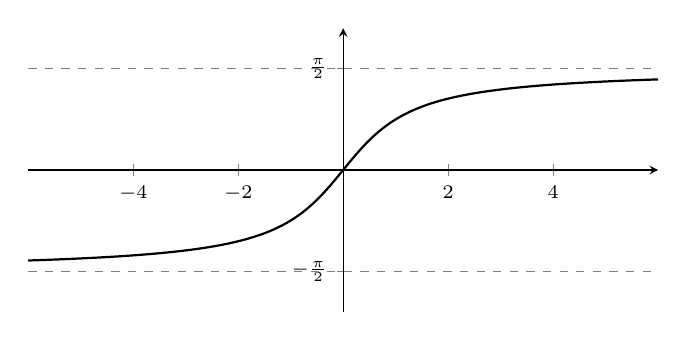
\begin{tikzpicture}
\begin{axis}[
  axis lines=middle,
  xmin=-6, xmax=6, ymin=-2.2, ymax=2.2,
  xtick={-4,-2,2,4},
  ytick={-1.5708,1.5708},
  yticklabels={$-\frac{\pi}{2}$,$\frac{\pi}{2}$},
  width=8cm, height=3.6cm, scale only axis,
  tick label style={font=\scriptsize},
]
\addplot[gray, dashed, domain=-6:6, samples=2] {1.5708};
\addplot[gray, dashed, domain=-6:6, samples=2] {-1.5708};
\addplot[thick, domain=-6:6, samples=120] {rad(atan(x))};
\end{axis}
\end{tikzpicture}
\end{center}

\begin{proposition}{逆三角関数の微分}{tb-inverse-trig-derivative}
\[
(\arcsin x)'=\frac1{\sqrt{1-x^2}},\qquad
(\arccos x)'=-\frac1{\sqrt{1-x^2}},\qquad
(\arctan x)'=\frac1{1+x^2}.
\]
\end{proposition}

\begin{proof}
公式は覚えなくても、その場で作れる。
$\theta=\arcsin x$ とおくと $\sin\theta=x$ であり、両辺を $x$ で微分すると
\[
\cos\theta\cdot\frac{\d\theta}{\d x}=1,
\qquad\text{すなわち}\qquad
\frac{\d\theta}{\d x}=\frac1{\cos\theta}.
\]
分母の $\cos\theta$ を $x$ で表せばよい。斜辺が $1$、$\theta$ の対辺が $x$ の
直角三角形を描くと、残る辺は三平方の定理から $\sqrt{1-x^2}$ である。

\begin{center}
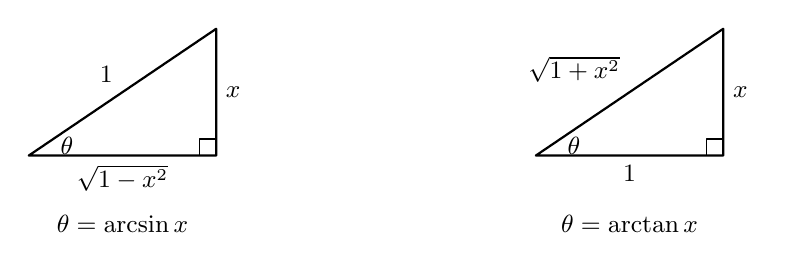
\begin{tikzpicture}[scale=1.4, line join=round]
\draw[thick] (0,0) -- (1.7,0) -- (1.7,1.15) -- cycle;
\draw (1.55,0) rectangle (1.7,0.15);
\node[below, font=\small] at (0.85,0) {$\sqrt{1-x^2}$};
\node[right, font=\small] at (1.7,0.575) {$x$};
\node[above left, font=\small] at (0.85,0.575) {$1$};
\node[right, font=\small] at (0.2,0.09) {$\theta$};
\node[font=\small] at (0.85,-0.62) {$\theta=\arcsin x$};
\begin{scope}[xshift=4.6cm]
\draw[thick] (0,0) -- (1.7,0) -- (1.7,1.15) -- cycle;
\draw (1.55,0) rectangle (1.7,0.15);
\node[below, font=\small] at (0.85,0) {$1$};
\node[right, font=\small] at (1.7,0.575) {$x$};
\node[above left, font=\small] at (0.85,0.575) {$\sqrt{1+x^2}$};
\node[right, font=\small] at (0.2,0.09) {$\theta$};
\node[font=\small] at (0.85,-0.62) {$\theta=\arctan x$};
\end{scope}
\end{tikzpicture}
\end{center}

主値では $-\pi/2\le\theta\le\pi/2$ なので $\cos\theta\ge0$ であり、
$\cos\theta=\sqrt{1-x^2}$ と符号が決まる。これで
$(\arcsin x)'=1/\sqrt{1-x^2}$ を得る。

$\arctan$ も同じ手順である。$\theta=\arctan x$ なら $\tan\theta=x$ で
\[
\sec^2\theta\cdot\frac{\d\theta}{\d x}=1,
\qquad
\frac{\d\theta}{\d x}=\frac1{\sec^2\theta}=\cos^2\theta.
\]
対辺が $x$、隣辺が $1$ の直角三角形では斜辺が $\sqrt{1+x^2}$ なので
$\cos\theta=1/\sqrt{1+x^2}$、従って $(\arctan x)'=1/(1+x^2)$ である。
\end{proof}

\begin{proposition}{$\arcsin$ と $\arccos$ の関係}{tb-arcsin-arccos}
$-1\le x\le1$ に対して
\[
\arcsin x+\arccos x=\frac\pi2.
\]
\end{proposition}

\begin{proof}
$\theta=\arcsin x$ とすると $\cos(\pi/2-\theta)=\sin\theta=x$ であり、
$-\pi/2\le\theta\le\pi/2$ から $0\le\pi/2-\theta\le\pi$ なので、
$\pi/2-\theta$ は $\arccos x$ の主値の範囲に入る。従って $\pi/2-\theta=\arccos x$ である。
\end{proof}

この式の両辺を微分すれば $(\arccos x)'=-(\arcsin x)'$ となる。
$\arccos$ の導関数が $\arcsin$ と符号だけ違うのは、
二つが $\pi/2$ を挟んで折り返しの関係にあるからである。

\section{双曲線関数}

\begin{definition}{双曲線関数}{tb-hyperbolic}
\[
\sinh x=\frac{e^x-e^{-x}}2,\qquad
\cosh x=\frac{e^x+e^{-x}}2,\qquad
\tanh x=\frac{\sinh x}{\cosh x}.
\]
\end{definition}

\begin{proposition}{双曲線関数の性質}{tb-hyperbolic-properties}
\[
\cosh^2x-\sinh^2x=1,
\qquad
(\sinh x)'=\cosh x,
\qquad
(\cosh x)'=\sinh x.
\]
また $\sinh$ の逆関数は
\[
\operatorname{arsinh}x=\log\left(x+\sqrt{x^2+1}\right)
\]
である。
\end{proposition}

\begin{example}{置換 $t=x+\sqrt{x^2+1}$}{tb-substitution-t}
$t=x+\sqrt{x^2+1}$ とおくと
\[
\left(\sqrt{x^2+1}+x\right)\left(\sqrt{x^2+1}-x\right)=(x^2+1)-x^2=1
\]
なので $t^{-1}=\sqrt{x^2+1}-x$ である。従って
\[
x=\frac{t-t^{-1}}2,\qquad
\sqrt{x^2+1}=\frac{t+t^{-1}}2,\qquad
\d x=\frac{1+t^{-2}}2\,\d t.
\]
これは $x=\sinh u$, $t=e^u$ と置いたことに他ならない。
$\sqrt{x^2+1}$ を含む積分は、この置換で有理式へ落ちる。
\end{example}

\begin{memo*}
2015年度 応用数理 専門基礎 第3問では、
$\int_0^1\d x/\sqrt{x^2+1}$ と $\int_0^1\sqrt{x^2+1}\,\d x$ を
まさにこの置換で計算する。$t$ と $t^{-1}$ を足し引きするところが要点である。
\end{memo*}

\section{よく使う不等式}

\begin{proposition}{基本不等式}{tb-basic-inequalities}
\[
\abs{\sin x}\le\abs x\quad(x\in\R),
\qquad
\abs{\sin x}\le1,
\]
\[
1+x\le e^x\quad(x\in\R),
\qquad
\log x\le x-1\quad(x>0).
\]
\end{proposition}

\begin{proposition}{相加平均・相乗平均}{tb-am-gm}
$u,v\ge0$ に対して
\[
uv\le\left(\frac{u+v}2\right)^2,
\qquad\text{すなわち}\qquad
\sqrt{uv}\le\frac{u+v}2
\]
であり、等号は $u=v$ のときに限る。
\end{proposition}

\begin{proposition}{三角不等式と Cauchy--Schwarz の不等式}{tb-triangle-cauchy}
実数・ベクトル・ノルムのいずれについても
\[
\abs{a+b}\le\abs a+\abs b,
\qquad
\bigl|\abs a-\abs b\bigr|\le\abs{a-b}
\]
が成り立つ。内積空間では
\[
\abs{\inner xy}\le\norm x\,\norm y
\]
であり、等号は $x,y$ が平行なときに限る。
\end{proposition}

「$\abs{A-B}\le C$ を示せ」という問題は、
まず $A\le B+C$ を示し、次に $A,B$ を入れ替えて $B\le A+C$ を示す、
という二段構えで書くのが定型である。
2026年度 第2期 専門基礎 第3問、2021年度 第2期 専門基礎 第3問、
年度不明の距離空間の問題はいずれもこの型である。

\section{覚えておく極限}

\begin{proposition}{標準的な極限}{tb-standard-limits}
\[
\lim_{x\to0}\frac{\sin x}x=1,
\qquad
\lim_{x\to0}\frac{1-\cos x}{x^2}=\frac12,
\qquad
\lim_{x\to0}\frac{e^x-1}x=1,
\]
\[
\lim_{x\to0}\frac{\log(1+x)}x=1,
\qquad
\lim_{n\to\infty}\left(1+\frac1n\right)^n=e,
\]
\[
\lim_{x\to\infty}\frac{\log x}{x^\alpha}=0\ (\alpha>0),
\qquad
\lim_{x\to\infty}\frac{x^\alpha}{e^x}=0,
\qquad
\lim_{x\to+0}x^\alpha\log x=0\ (\alpha>0).
\]
最後の三つは「対数は冪より遅く、冪は指数より遅い」と覚える。
\end{proposition}

これらの $x$ は、$0$ または $\infty$ へ向かう任意の式で置き換えてよい。
たとえば $h\to0$ のとき $x^2h\to0$ なので、$\lim_{x\to0}\sin x/x=1$ は
\[
\frac{\sin(x^2h)}{x^2h}\longrightarrow1
\]
の形で使える。置き換えた式が本当に $0$ または $\infty$ へ向かうことを、
使う前に確かめること。

\begin{memo*}
$\sin x/x\to1$ は、2021年度 第1期 専門基礎 第2問の偏微分の計算と、
2015年度 専門科目 第7問の優収束定理の適用で使う。
$\log x/x^\alpha\to0$ は、2015年度 第1期 専門基礎 第2問で
広義積分 $\int_1^\infty u^a\log u\,\d u$ の収束を判定するときに使う。
\end{memo*}
